\section{Shading}

Shading is a process that is often applied to 3D rendered objects to make them appear more realistic by modeling  how light interacts with them. In the code we have implemented, we have used the Equation \ref{eq:shading}. In the equation \textit{I} is final illuminated texture of a face, \textit{T(u, v)} is the texture of the face with dimensions s and t. \textit{L\textsubscript{a}} is the ambient illumination, \textit{k\textsubscript{a}} is the ambient component of the object's material. \textit{L\textsubscript{l}} is light intensity, \textit{k\textsubscript{d}} is the diffuse component of the material. \textit{n} is the face normal vector. \textit{k\textsubscript{s}} is the specular component of the material. \textit{v} is the viewer vector and \textit{r\textsubscript{i}} is the reflected light vector. All vectors are unitary.

\begin{equation}
	I=T(u,v)[
	\underbrace{
	L_{a}k_{a}
	}_\text{Ambient}
	+
	\underbrace{
	k_{d}\sum\limits_{i}L_{i}max(n\cdot l_{i},0)
	}_\text{Diffuse}
	+
	\underbrace{
	k_{s}\sum\limits_{i}L_{i}(r_{i}\cdot v)^\alpha
	  }_\text{Specular}
	]
	\label{eq:shading}
\end{equation}

This equation differs slightly from what has been implemented in our report, because it allows for multiple light sources, whereas we have only implemented one light source. On the other hand both the equation, and our implementation assume the material is uniform, while it could easily be a texture.

To shade the individual faces in our project, we used a low resolution (10$\times$10) texture that we have multiplied with the texture calculated from before. We have implemented two different approaches to shading, the flat shading model and and Phong shading model. In both models, the underlying equation is the same (Figure \ref{eq:shading}), but there are differences in how it is applied.

In the flat shading model, we only need to calculate one diffuse and specular value per face, and apply it to the whole face.

In contrast, Phong shading model assigns each pixel in our light texture a different normal, calculated using bilinear interpolation from corner normals of the currently evaluated face. The corner normals are calculated by averaging the normals of all neighboring faces. The result of all of this is that there is a smooth transition between normals calculated for points along the face. This allows us to draw objects with relatively small face counts (and therefore smaller and easier to store and manipulate) easily and with nice smooth surface. 

This means that we can then use this normal to calculate the illumination at a single point of the face texture to obtain a smooth gradient corresponding to diffuse and specular light. 

All that remains is then to combine the illumination texture with the original texture to shade the face and project it to create the final image. Of course this is repeated for every face.

We have also implemented different light positions. It is possible to click into the camera window and select a new position for the light, which is by default positioned in the camera center, see Figure \ref{subfig:extra1} and \ref{subfig:extra2}. 

 \begin{figure}[h!]
	\begin{subfigure}[b]{0.5\textwidth}
		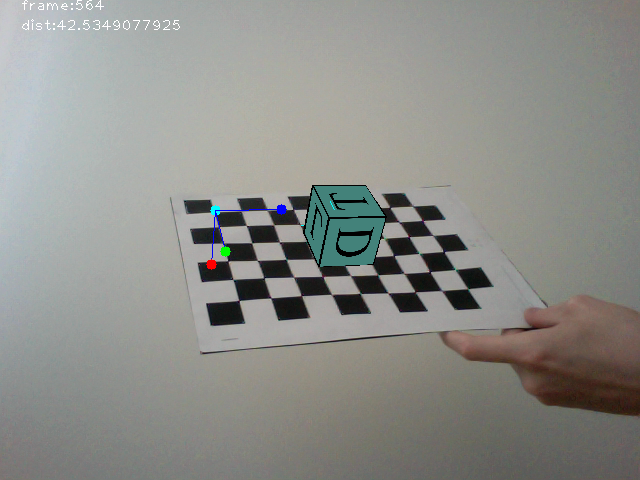
\includegraphics[width=\textwidth]{Handin3/images/texture2.png}
		\caption{Plain Texture Mapping}
		\label{subfig:plaintexture}
	\end{subfigure}
	~
	\begin{subfigure}[b]{0.5\textwidth}
		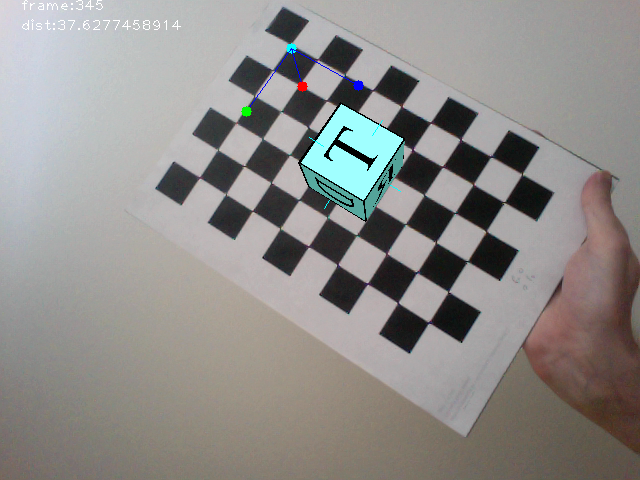
\includegraphics[width=\textwidth]{Handin3/images/flat.png}
		\caption{Flat Shading}
		\label{subfig:flatshading}
	\end{subfigure}
	~
	\begin{subfigure}[b]{0.5\textwidth}
		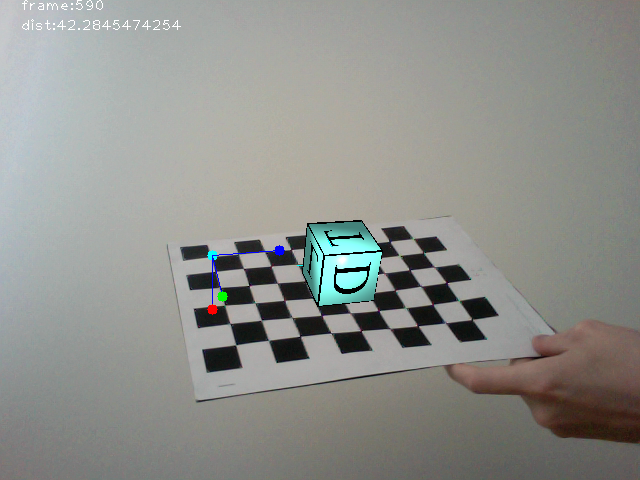
\includegraphics[width=\textwidth]{Handin3/images/phong1.png}
		\caption{Phong Shading}
		\label{subfig:phongshading}
	\end{subfigure}
	~
	\begin{subfigure}[b]{0.5\textwidth}
		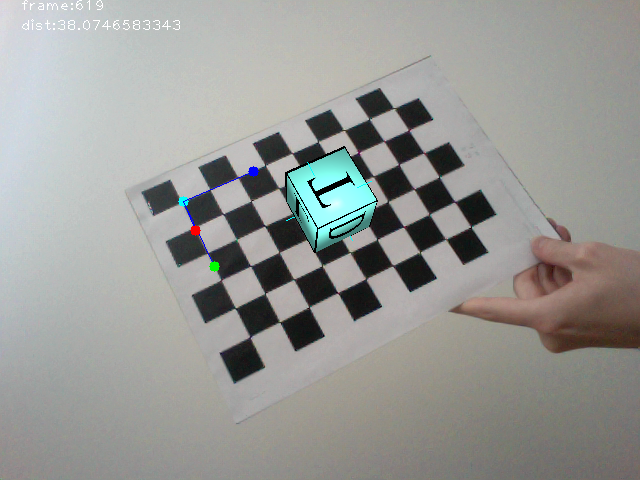
\includegraphics[width=\textwidth]{Handin3/images/phong2.png}
		\caption{Phong Shading 2}
		\label{subfig:phongshading2}
	\end{subfigure}
	~
	\begin{subfigure}[b]{0.5\textwidth}
		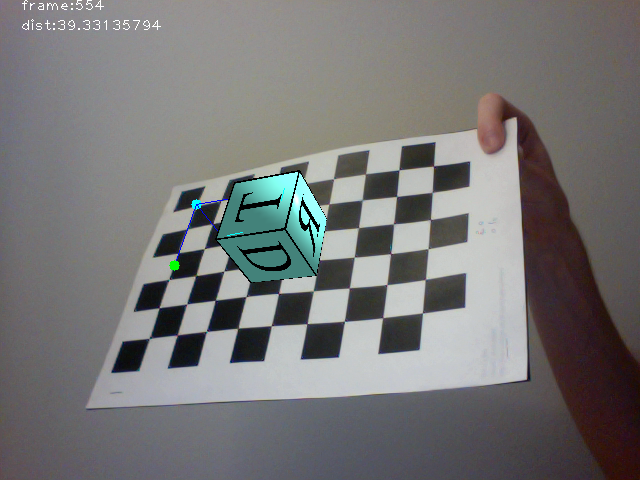
\includegraphics[width=\textwidth]{Handin3/images/extra1.png}
		\caption{Light Position Top Right}
		\label{subfig:extra1}
	\end{subfigure}
	~
	\begin{subfigure}[b]{0.5\textwidth}
		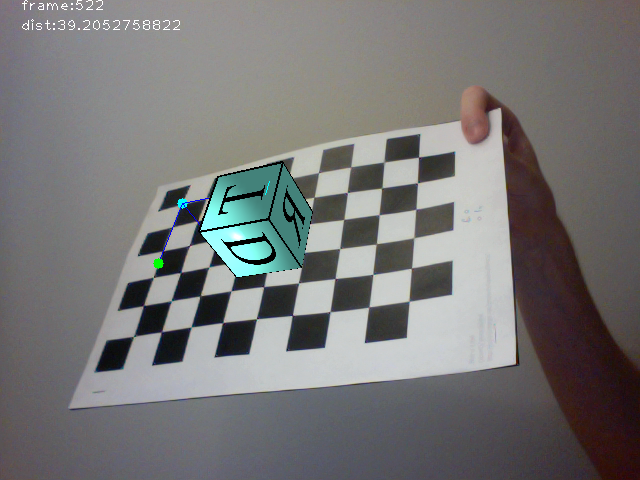
\includegraphics[width=\textwidth]{Handin3/images/extra2.png}
		\caption{Light Position Bottom Left}
		\label{subfig:extra2}
	\end{subfigure}
	
	\label{fig:texturing}
	\caption{Shading}
\end{figure}